% Provenance (never printed): cycle 3 "La planete Terre" and geography
% (weather and climate; reading a climate chart; the great climate zones of
% the world, hot, temperate and cold); see sources/book1/PROVENANCE.md.
% Book 1, grade 5, chapter 2.
\chapter{Tempo e clima}\label{ch:g5:weather-and-climate}

Na segunda semana de janeiro, chegam dois cartões-postais à escola. O
primeiro, da prima de Lena, mostra crianças fazendo um castelo de \omterm{def:g3:stones-pebbles-sand:sand}{areia}
numa praia ensolarada, embaixo de coqueiros. O segundo, da avó de Tom,
mostra crianças fazendo um boneco de \omterm{def:g4:clouds-rain-snow:precipitation}{neve} num jardim coberto de \omterm{def:g4:clouds-rain-snow:precipitation}{neve}.
``Como pode ser verão e inverno na mesma semana?'', pergunta Tom.

Não é o \omterm{def:g1:watching-the-weather:weather}{tempo} de um dia que muda tanto de um lugar para o outro. É o \omterm{def:g1:watching-the-weather:weather}{tempo}
que eles têm, ano após ano: o seu \omterm{def:g5:weather-and-climate:climate}{clima}.

\begin{omfigure}
\begin{minipage}[b]{0.48\linewidth}\centering

\includegraphics[width=\linewidth]{images/book1/ai/g5-beach-postcard.jpg}
\end{minipage}\hfill
\begin{minipage}[b]{0.48\linewidth}\centering

\includegraphics[width=\linewidth]{images/book1/ai/g5-snowman-postcard.jpg}
\end{minipage}

{\small Dois cartões-postais da mesma semana de janeiro: uma praia
ensolarada e um jardim coberto de \omterm{def:g4:clouds-rain-snow:precipitation}{neve}.}
\end{omfigure}

\begin{recall}
O \omterm{def:g1:watching-the-weather:weather}{tempo} é o estado do ar num lugar e num momento: ensolarado, nublado,
chuvoso, com \omterm{def:g4:clouds-rain-snow:precipitation}{neve}, com vento (\cref{ch:g1:watching-the-weather}). O
termômetro mede a temperatura do ar, em graus Celsius; o \omterm{def:g4:clouds-rain-snow:rain-gauge}{pluviômetro} mede
a \omterm{def:g4:clouds-rain-snow:precipitation}{chuva}, em milímetros (\cref{ch:g4:clouds-rain-snow}). O \omterm{def:g3:continents-and-oceans:equator}{equador} dá a
volta no meio do \omterm{def:g3:continents-and-oceans:globe}{globo}, a meio caminho entre o \omterm{def:g3:continents-and-oceans:poles}{Polo Norte} e o \omterm{def:g3:continents-and-oceans:poles}{Polo Sul}
(\cref{ch:g3:continents-and-oceans}). Os livros de física mostraram que a
Terra dá uma volta em torno do Sol em um ano, e que as suas estações vêm
da inclinação do seu eixo: no verão, o Sol sobe mais alto no céu e os dias
são mais longos.
\end{recall}

\section{O tempo é o de hoje, o clima é o de costume}

O \omterm{def:g1:watching-the-weather:weather}{tempo} muda de um dia para o outro, e até de uma hora para a outra. O
\omterm{def:g5:weather-and-climate:climate}{clima} é outra coisa.

\begin{definition}[Clima]\label{def:g5:weather-and-climate:climate}
O \emph{clima}\index{clima} de um lugar é o \omterm{def:g1:watching-the-weather:weather}{tempo} que ele costuma ter, mês
a mês, ao longo de muitos anos: quão quente ou frio, quão úmido ou seco é
cada estação. Os meteorologistas o calculam fazendo a média das medições
de 30 anos.
% ledger: wmo:normal-30yr
\end{definition}

``Está chovendo hoje de manhã'' é uma frase sobre o \omterm{def:g1:watching-the-weather:weather}{tempo}. ``Aqui chove
muito no outono'' é uma frase sobre o \omterm{def:g5:weather-and-climate:climate}{clima}. Um único dia frio no verão
não muda o \omterm{def:g5:weather-and-climate:climate}{clima}: é só um \omterm{def:g1:watching-the-weather:weather}{tempo} fora do comum.

Os meteorologistas do mundo inteiro usam a mesma regra: eles fazem a média
de 30 anos de medições. As médias usadas hoje são as dos anos de 1991 a
2020.
% ledger: wmo:normal-30yr

\section{O climograma}

Para mostrar o \omterm{def:g5:weather-and-climate:climate}{clima} de um lugar numa só imagem, desenhamos um gráfico.

\begin{definition}[Climograma]\label{def:g5:weather-and-climate:climate-chart}
Um \emph{climograma}\index{climograma} mostra, para cada mês do ano, a
temperatura média de um lugar (uma curva) e a quantidade média de \omterm{def:g4:clouds-rain-snow:precipitation}{chuva} e
de \omterm{def:g4:clouds-rain-snow:precipitation}{neve} que cai ali (barras, em milímetros de água).
\end{definition}

\begin{omfigure}
\begin{tikzpicture}
  \begin{axis}[name=pax, width=0.55\linewidth, height=5.6cm, ymin=0, ymax=400,
      axis y line*=right, axis x line=none, ybar, bar width=7pt,
      ytick={0,100,...,400}, ylabel={chuva (mm)}, xmin=0.4, xmax=12.6,
      tick label style={font=\scriptsize}, label style={font=\scriptsize},
      ylabel style={blue!60!black}]
    \addplot[fill=blue!40, draw=blue!60!black]
      table[x=month, y=prcp_mm] {figdata/out/grade-5-climate_charts-seattle.dat};
  \end{axis}
  \begin{axis}[width=0.55\linewidth, height=5.6cm, ymin=-30, ymax=40,
      axis y line*=left, axis x line*=bottom, xmin=0.4, xmax=12.6,
      xtick={1,...,12}, xticklabels={J,F,M,A,M,J,J,A,S,O,N,D},
      ytick={-30,-20,...,40}, ylabel={temperatura ($^\circ$C)},
      tick label style={font=\scriptsize}, label style={font=\scriptsize},
      ylabel style={red!70!black}]
    \addplot[red!70!black, thick, mark=*, mark size=1.3pt]
      table[x=month, y=tavg_C] {figdata/out/grade-5-climate_charts-seattle.dat};
    \draw[gray!60] (axis cs:0.4,0) -- (axis cs:12.6,0);
    \begin{scope}[every node/.style={circle, draw, fill=white, inner sep=0.8pt,
        font=\scriptsize\bfseries}]
      \node[text=red!70!black, draw=red!70!black] at (axis cs:5.5,27) {1};
      \node[text=blue!60!black, draw=blue!60!black] at (axis cs:7,-19) {2};
    \end{scope}
  \end{axis}
  \node[anchor=north west, font=\scriptsize, align=left, text width=4.2cm]
    at ($(pax.outer north east)+(0.3,-0.1)$) {%
    \textcolor{red!70!black}{\textbf{1} A curva vermelha: a temperatura média
    de cada mês, lida na escala da esquerda.}\par\smallskip
    \textcolor{blue!60!black}{\textbf{2} As barras azuis: a chuva média de cada
    mês, lida na escala da direita.}\par\smallskip
    \textbf{3} As letras embaixo do gráfico: os meses, de janeiro a
    dezembro.};
\end{tikzpicture}

{\small O \omterm{def:g5:weather-and-climate:climate-chart}{climograma} de Seattle, uma cidade da costa oeste dos Estados
Unidos. Médias dos anos de 1991 a 2020 (dados: NOAA).}
% ledger: data:b1-noaa-normals
\end{omfigure}

\begin{method}[Ler um climograma]\label{met:g5:weather-and-climate:reading}
\begin{enumerate}
  \item Encontre o mês mais quente e o mais frio na curva vermelha, e leia
        as suas temperaturas na escala da esquerda. A curva é plana (a
        mesma temperatura o ano todo) ou ela sobe e desce (estações quentes
        e frias)? Ela desce abaixo de 0~$^\circ$C (geada)?
  \item Encontre o mês mais chuvoso e o mais seco entre as barras azuis, e
        leia-os na escala da direita. As barras são altas ou baixas? Há uma
        estação seca?
  \item Junte tudo numa frase: ``quente e seco o ano todo'', ``ameno e
        chuvoso, com um verão seco''{\ldots}
\end{enumerate}
\end{method}

\begin{example}[Seattle]\label{ex:g5:weather-and-climate:seattle}
Em Seattle, o mês mais quente é agosto (cerca de 20~$^\circ$C) e o mais
frio é dezembro (cerca de 6~$^\circ$C): a curva sobe e desce, mas nunca
fica abaixo do ponto de congelamento. A barra mais alta é a de novembro
(cerca de 160~mm), a mais baixa a de julho (cerca de 15~mm). Numa frase:
invernos amenos, verões frescos, chuvoso no outono e no inverno, bastante
seco no verão. Num ano inteiro caem cerca de 1\,000~milímetros de \omterm{def:g4:clouds-rain-snow:precipitation}{chuva}:
um metro de água.
% ledger: data:b1-noaa-normals
\end{example}

\section{Quatro climas}

Aqui estão os \omterm{def:g5:weather-and-climate:climate-chart}{climogramas} de quatro cidades dos Estados Unidos, longe umas
das outras: Phoenix, no \omterm{def:g5:weather-and-climate:desert}{deserto} do Arizona; Hilo, na ilha do Havaí, no meio
do \omterm{def:g2:water-on-earth:ocean}{oceano} Pacífico; Seattle, na costa oeste; e Utqiaġvik, no extremo norte
do Alasca, no \omterm{def:g1:landscapes-around-us:water}{litoral} do \omterm{def:g2:water-on-earth:ocean}{oceano} Ártico. Os quatro gráficos usam as mesmas
escalas, então podemos compará-los num piscar de olhos.

\begin{omfigure}
\def\gfivechart#1#2{%
\begin{tikzpicture}
  \begin{axis}[width=0.5\linewidth, height=4.6cm, ymin=0, ymax=400,
      axis y line*=right, axis x line=none, ybar, bar width=4pt,
      ytick={0,100,...,400}, xmin=0.4, xmax=12.6,
      tick label style={font=\tiny}]
    \addplot[fill=blue!40, draw=blue!60!black]
      table[x=month, y=prcp_mm] {figdata/out/grade-5-climate_charts-#1.dat};
  \end{axis}
  \begin{axis}[width=0.5\linewidth, height=4.6cm, ymin=-30, ymax=40,
      axis y line*=left, axis x line*=bottom, xmin=0.4, xmax=12.6,
      xtick={1,...,12}, xticklabels={J,F,M,A,M,J,J,A,S,O,N,D},
      ytick={-30,-20,...,40}, tick label style={font=\tiny},
      title={#2}, title style={font=\scriptsize\bfseries, yshift=-4pt}]
    \addplot[red!70!black, thick, mark=*, mark size=1pt]
      table[x=month, y=tavg_C] {figdata/out/grade-5-climate_charts-#1.dat};
    \draw[gray!60] (axis cs:0.4,0) -- (axis cs:12.6,0);
  \end{axis}
\end{tikzpicture}}%
\gfivechart{phoenix}{Phoenix: um \omterm{def:g5:weather-and-climate:desert}{deserto} quente}\hfill
\gfivechart{hilo}{Hilo: um \omterm{def:g5:weather-and-climate:climate}{clima} de \omterm{def:g5:weather-and-climate:rainforest}{floresta tropical úmida}}

\medskip
\gfivechart{seattle}{Seattle: um \omterm{def:g5:weather-and-climate:climate}{clima} temperado}\hfill
\gfivechart{utqiagvik}{Utqiaġvik: um \omterm{def:g5:weather-and-climate:climate}{clima} polar}

{\small Quatro \omterm{def:g5:weather-and-climate:climate-chart}{climogramas} com as mesmas escalas: a temperatura em
$^\circ$C à esquerda (curva vermelha), a \omterm{def:g4:clouds-rain-snow:precipitation}{chuva} em milímetros à direita
(barras azuis). Médias dos anos de 1991 a 2020 (dados: NOAA).}
% ledger: data:b1-noaa-normals
\end{omfigure}

\paragraph{O deserto.} Em Phoenix, as barras são tão baixas que mal dá para
vê-las: num ano inteiro, caem menos de 200 milímetros de \omterm{def:g4:clouds-rain-snow:precipitation}{chuva}. Os verões
são muito quentes: em julho, a temperatura média é de 35 graus.
% ledger: data:b1-noaa-normals

\begin{definition}[Deserto]\label{def:g5:weather-and-climate:desert}
Um \emph{deserto}\index{deserto} é um lugar onde cai muito pouca \omterm{def:g4:clouds-rain-snow:precipitation}{chuva}:
menos de 250 milímetros num ano. Poucas plantas conseguem viver ali, e o
chão muitas vezes fica descoberto.
% ledger: usgs:arid-250mm
\end{definition}

Os \omterm{def:g5:weather-and-climate:desert}{desertos} nem sempre são quentes. Veja Utqiaġvik: ali caem menos de
150 milímetros num ano, ainda menos que em Phoenix: é um \omterm{def:g5:weather-and-climate:desert}{deserto} frio. Os
\omterm{def:g5:weather-and-climate:desert}{desertos} podem ser quentes ou frios.
% ledger: data:b1-noaa-normals, usgs:arid-250mm

\paragraph{A floresta tropical úmida.} Hilo é o contrário de Phoenix. As
suas barras são as mais altas dos quatro gráficos: caem mais de
3\,000 milímetros de \omterm{def:g4:clouds-rain-snow:precipitation}{chuva} num ano, e todos os meses são chuvosos. E a sua
curva vermelha é quase plana: entre 22 e 25 graus o ano todo. Não existe
inverno nenhum.
% ledger: data:b1-noaa-normals

\begin{definition}[Floresta tropical úmida]\label{def:g5:weather-and-climate:rainforest}
Uma \emph{floresta tropical úmida}\index{floresta tropical umida@floresta tropical úmida} é uma floresta
densa de árvores muito altas que cresce onde faz calor e é úmido o ano
todo, com \omterm{def:g4:clouds-rain-snow:precipitation}{chuvas} fortes em todos os meses. A maioria das florestas
tropicais úmidas fica perto do \omterm{def:g3:continents-and-oceans:equator}{equador}.
\end{definition}

\begin{omfigure}
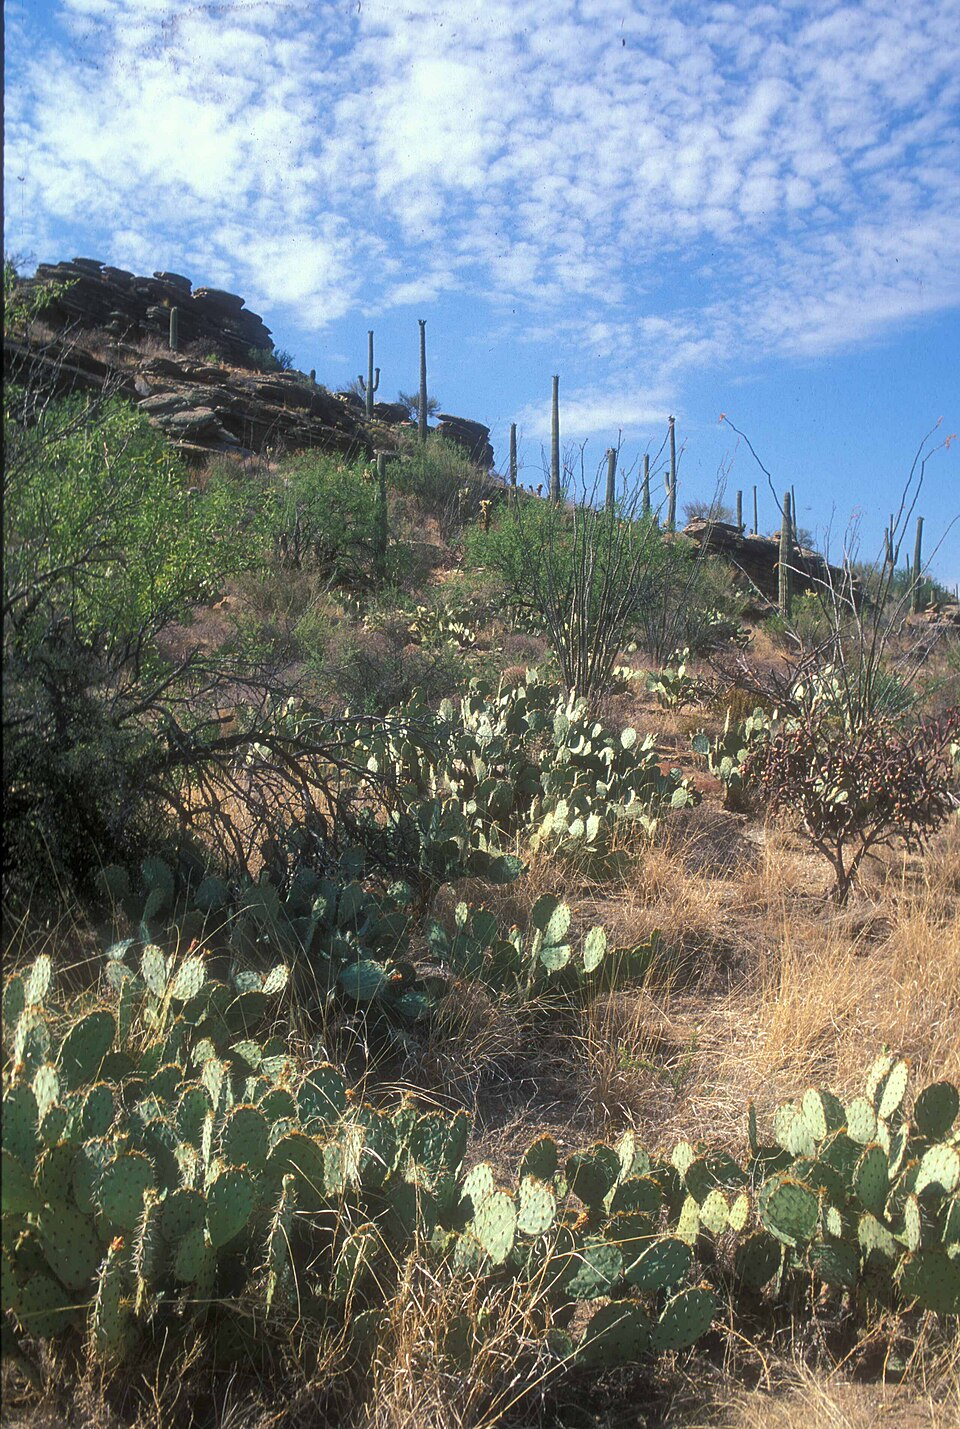
\includegraphics[height=3.6cm]{images/book1/g5-sonoran-desert.jpg}\quad
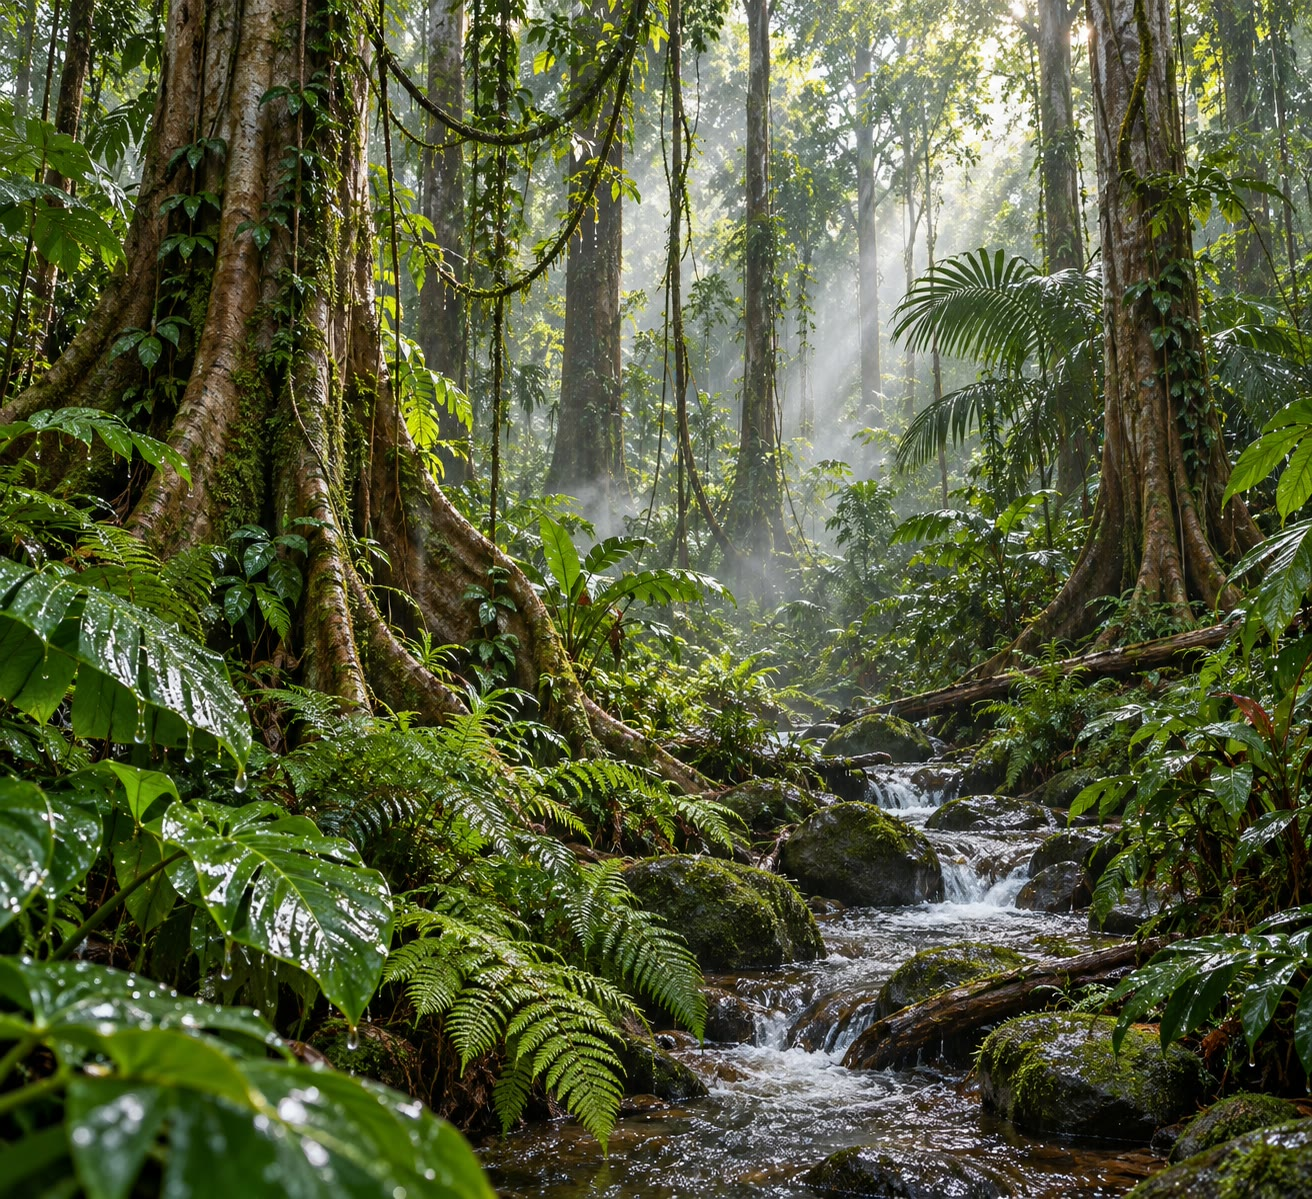
\includegraphics[height=3.6cm]{images/book1/ai/g5-rainforest.jpg}\quad
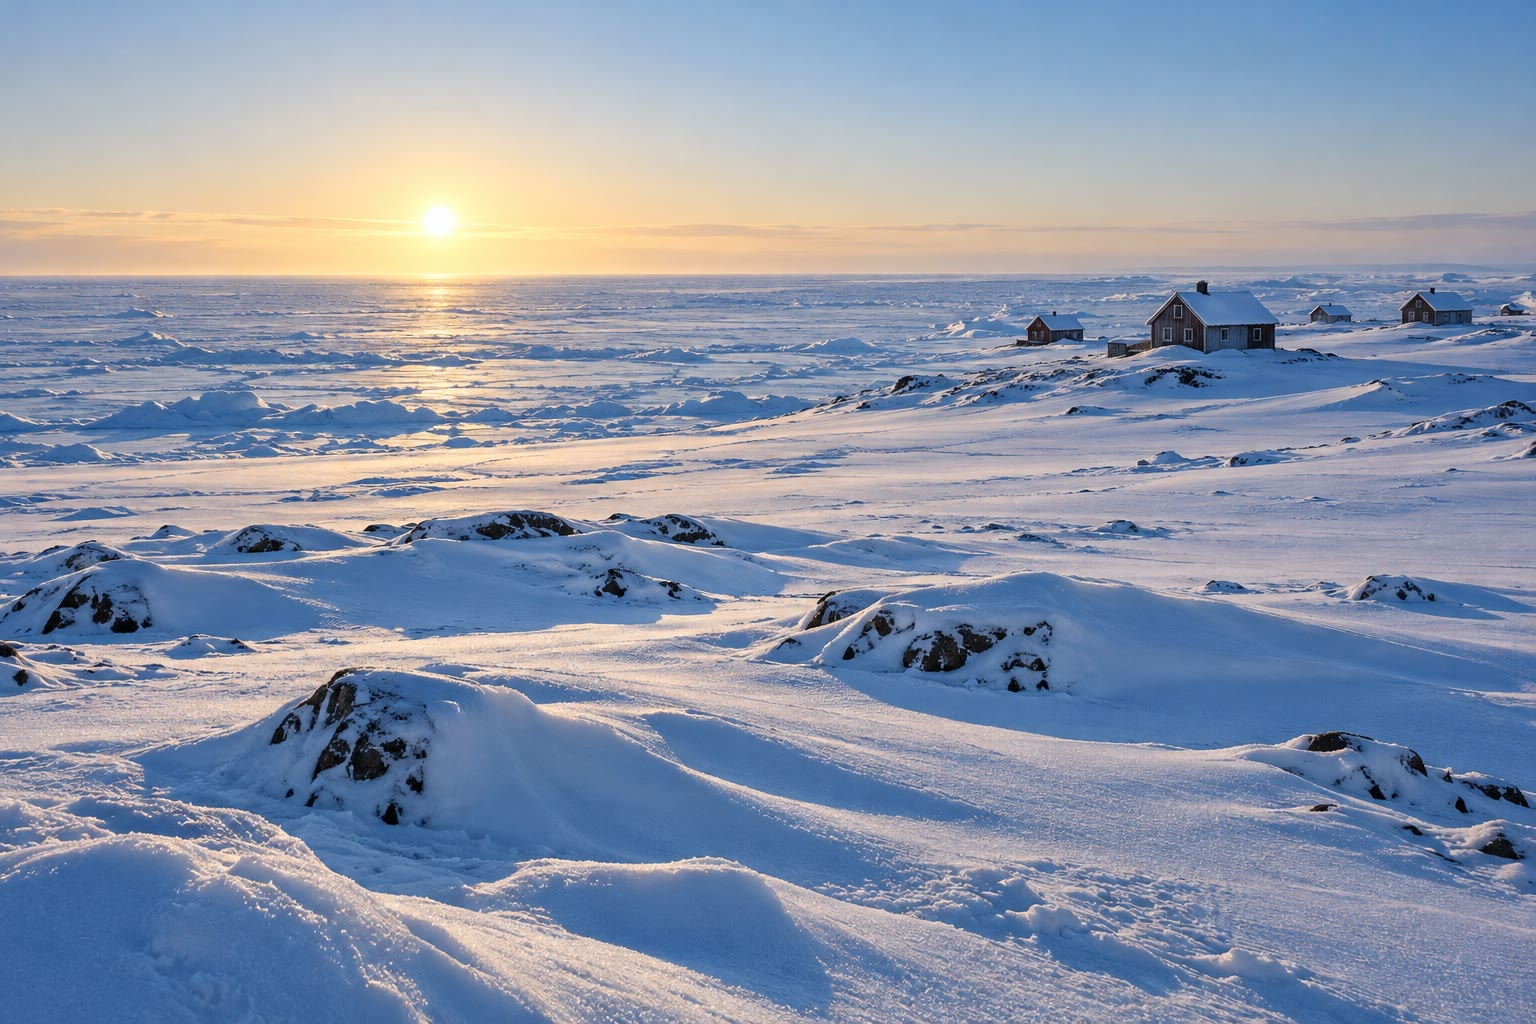
\includegraphics[height=3.6cm]{images/book1/ai/g5-polar-tundra.jpg}

{\small Três \omterm{def:g5:weather-and-climate:climate}{climas} extremos. À esquerda: o \omterm{def:g5:weather-and-climate:desert}{deserto} de Sonora, no Arizona,
o \omterm{def:g5:weather-and-climate:desert}{deserto} de Phoenix, com cactos saguaro altos e palmas, que guardam água
nos seus caules grossos (fotografia: U.S. National Park Service, Saguaro
National Park, domínio público). No meio: dentro de uma \omterm{def:g5:weather-and-climate:rainforest}{floresta tropical
úmida} depois de um aguaceiro. À direita: um \omterm{def:g1:landscapes-around-us:water}{litoral} polar no inverno, com
o \omterm{def:g2:water-on-earth:ocean}{mar} congelado e o Sol baixo ao meio-dia.}
% ledger: nps:sonoran-desert
\end{omfigure}

\paragraph{O clima temperado.} Seattle fica no meio-termo: a sua curva sobe
no verão e desce no inverno, mas nunca muito; chove bastante, sobretudo no
outono e no inverno. É um \omterm{def:g5:weather-and-climate:climate}{clima} temperado: nem muito calor, nem muito frio.

\paragraph{O clima polar.} Em Utqiaġvik, a curva vermelha fica abaixo de
0~$^\circ$C durante oito meses do ano; em fevereiro, a média é de 24 graus
abaixo de zero. Mesmo em julho, o mês mais quente, faz só cerca de
5 graus.
% ledger: data:b1-noaa-normals

\section{Zonas quentes, temperadas e frias}

Por que faz calor perto do \omterm{def:g3:continents-and-oceans:equator}{equador} e frio perto dos \omterm{def:g3:continents-and-oceans:poles}{polos}? Por causa do
Sol. Perto do \omterm{def:g3:continents-and-oceans:equator}{equador}, o Sol do meio-dia fica alto no céu o ano todo: a
sua luz cai quase reta e esquenta muito o chão. Perto dos \omterm{def:g3:continents-and-oceans:poles}{polos}, o Sol
fica sempre baixo: a sua luz chega inclinada, espalhada por uma área
grande, e esquenta pouco. No inverno, ali, o Sol pode nem nascer.

Dois pares de linhas em volta do \omterm{def:g3:continents-and-oceans:globe}{globo} dividem a Terra em \omterm{def:g5:weather-and-climate:climate-zone}{zonas climáticas}.

\begin{definition}[Trópicos e círculos polares]\label{def:g5:weather-and-climate:tropics}
Os dois \emph{trópicos}\index{tropico@trópico} são as linhas em volta do \omterm{def:g3:continents-and-oceans:globe}{globo}, uma
ao norte e outra ao sul do \omterm{def:g3:continents-and-oceans:equator}{equador}, que marcam até que distância do
\omterm{def:g3:continents-and-oceans:equator}{equador} o Sol do meio-dia pode ficar bem a pino: o trópico de Câncer, no
norte, e o trópico de Capricórnio, no sul. Os dois \emph{círculos
polares}\index{circulo polar@círculo polar} são as linhas em volta do \omterm{def:g3:continents-and-oceans:globe}{globo}, perto dos
\omterm{def:g3:continents-and-oceans:poles}{polos}, além das quais, no meio do inverno, o Sol não nasce durante pelo
menos um dia, e, no meio do verão, ele não se põe: o Círculo Polar Ártico,
no norte, e o Círculo Polar Antártico, no sul.
\end{definition}

A inclinação do eixo da Terra decide onde ficam essas linhas.

\begin{definition}[Zonas climáticas]\label{def:g5:weather-and-climate:climate-zone}
A Terra é dividida em três tipos de \emph{zona climática}\index{zona climatica@zona climática}: a \emph{zona quente}, entre os dois \omterm{def:g5:weather-and-climate:tropics}{trópicos}, em volta do \omterm{def:g3:continents-and-oceans:equator}{equador};
as duas \emph{zonas temperadas}, entre um \omterm{def:g5:weather-and-climate:tropics}{trópico} e um \omterm{def:g5:weather-and-climate:tropics}{círculo polar}, onde
os verões e os invernos são diferentes; e as duas \emph{zonas frias}, além
dos \omterm{def:g5:weather-and-climate:tropics}{círculos polares}, em volta dos \omterm{def:g3:continents-and-oceans:poles}{polos}.
\end{definition}

\begin{omfigure}
\begin{tikzpicture}
\begin{axis}[ommap, width=\linewidth, xtick=\empty, ytick=\empty, grid=none,
    axis background/.style={fill=white}, clip=true]
  \addplot[fill=orange!35, draw=none] table {figdata/out/grade-5-climate_zones-hot.dat};
  \addplot[fill=green!20, draw=none] table {figdata/out/grade-5-climate_zones-temperate.dat};
  \addplot[fill=cyan!20, draw=none] table {figdata/out/grade-5-climate_zones-cold.dat};
  \addplot[fill=black!25, fill opacity=0.8, draw=black!60, line width=0.2pt]
    table {figdata/out/shared-geo-land.dat};
  \addplot[black!70, dashed, line width=0.5pt] table {figdata/out/grade-5-climate_zones-lines.dat};
  \draw[black!70, line width=0.6pt] (axis cs:-180,0) -- (axis cs:180,0);
  \addplot[only marks, mark=*, mark size=1.8pt, red!80!black]
    table[x=lon, y=lat] {figdata/out/grade-5-climate_zones-stations.dat};
  \begin{scope}[every node/.style={font=\scriptsize, fill=white, fill opacity=0.75,
      text opacity=1, inner sep=1pt}]
    \node[anchor=west] at (axis cs:-107,33.4) {Phoenix};
    \node[anchor=east] at (axis cs:-158,19.7) {Hilo};
    \node[anchor=west] at (axis cs:-117,47.4) {Seattle};
    \node[anchor=west] at (axis cs:-151,73.5) {Utqiaġvik};
  \end{scope}
  \begin{scope}[every node/.style={font=\scriptsize\bfseries, align=center,
      fill=white, fill opacity=0.7, text opacity=1, inner sep=1pt}]
    \node at (axis cs:-5,83) {zona fria};
    \node at (axis cs:-40,40) {zona temperada};
    \node at (axis cs:-25,-8) {zona quente};
    \node at (axis cs:95,-45) {zona temperada};
    \node at (axis cs:-60,-80) {zona fria};
  \end{scope}
\end{axis}
\end{tikzpicture}

{\small As \omterm{def:g5:weather-and-climate:climate-zone}{zonas climáticas}. De cima para baixo, as linhas tracejadas são
o Círculo Polar Ártico, o \omterm{def:g5:weather-and-climate:tropics}{trópico} de Câncer, o \omterm{def:g5:weather-and-climate:tropics}{trópico} de Capricórnio e o
Círculo Polar Antártico; a linha contínua é o \omterm{def:g3:continents-and-oceans:equator}{equador}. Os pontos vermelhos
são as quatro cidades dos \omterm{def:g5:weather-and-climate:climate-chart}{climogramas} acima.}
% ledger: earth:obliquity, data:b1-noaa-normals
\end{omfigure}

As zonas dão uma primeira ideia, aproximada. Dentro de cada uma, muitas
outras coisas mudam o \omterm{def:g5:weather-and-climate:climate}{clima}: a distância de um lugar até o \omterm{def:g2:water-on-earth:ocean}{mar}, a sua
\omterm{def:g4:world-physical-map:altitude}{altitude}, de onde vêm os seus ventos. Você vai conhecê-las nos próximos
anos.

\begin{remark}[Phoenix e as zonas]\label{rem:g5:weather-and-climate:phoenix}
No \omterm{def:g2:drawing-to-map:map}{mapa} das zonas, Phoenix fica um pouco ao norte do \omterm{def:g5:weather-and-climate:tropics}{trópico} de Câncer, na
zona temperada, e mesmo assim é um \omterm{def:g5:weather-and-climate:desert}{deserto} quente. As zonas são uma
primeira ideia, aproximada: muitos dos grandes \omterm{def:g5:weather-and-climate:desert}{desertos} quentes ficam perto
dos \omterm{def:g5:weather-and-climate:tropics}{trópicos}, na borda da zona quente, e você vai aprender por quê no
\cref{ch:g8:winds-global-circulation}.
\end{remark}

\section{Exercícios}

\begin{exercise}[$\star$]\label{exo:g5:weather-and-climate:1}
\omterm{def:g1:watching-the-weather:weather}{Tempo} ou \omterm{def:g5:weather-and-climate:climate}{clima}?
\begin{enumerate}
  \item[(a)] Está nevando em Utqiaġvik hoje de manhã.
  \item[(b)] Em Phoenix, os verões são muito quentes e secos.
  \item[(c)] Ontem à tarde soprou um vento forte em Seattle.
  \item[(d)] Em Hilo, chove muito em todos os meses do ano.
\end{enumerate}
\end{exercise}

\begin{exercise}[$\star$]\label{exo:g5:weather-and-climate:2}
O que é o \omterm{def:g5:weather-and-climate:climate}{clima} de um lugar? De quantos anos os meteorologistas fazem a
média das medições para descrevê-lo?
\end{exercise}

\begin{exercise}[$\star$]\label{exo:g5:weather-and-climate:3}
No \omterm{def:g5:weather-and-climate:climate-chart}{climograma} de Seattle, qual é o mês mais frio? Qual é o mês mais
chuvoso? A temperatura chega a ficar abaixo de 0~$^\circ$C?
\end{exercise}

\begin{exercise}[$\star$]\label{exo:g5:weather-and-climate:4}
No \omterm{def:g5:weather-and-climate:climate-chart}{climograma} de Utqiaġvik, qual é o mês mais quente? Algum mês passa de
10~$^\circ$C?
\end{exercise}

\begin{exercise}[$\star$]\label{exo:g5:weather-and-climate:5}
Em que \omterm{def:g5:weather-and-climate:climate-zone}{zona climática} fica cada um destes lugares: o \omterm{def:g3:continents-and-oceans:equator}{equador}; o \omterm{def:g3:continents-and-oceans:poles}{Polo
Norte}; um lugar a meio caminho entre o \omterm{def:g3:continents-and-oceans:equator}{equador} e o \omterm{def:g3:continents-and-oceans:poles}{Polo Sul}?
\end{exercise}

\begin{exercise}[$\star$]\label{exo:g5:weather-and-climate:6}
Use o \omterm{def:g2:drawing-to-map:map}{mapa} das zonas. Em que \omterm{def:g5:weather-and-climate:climate-zone}{zona climática} fica cada uma das quatro
cidades: Phoenix, Hilo, Seattle, Utqiaġvik?
\end{exercise}

\begin{exercise}[$\star\star$]\label{exo:g5:weather-and-climate:7}
Aqui está a \omterm{def:g4:clouds-rain-snow:precipitation}{chuva} média de cada mês em Seattle, em milímetros, arredondada
para números inteiros:
\begin{center}
\begin{tabular}{|*{12}{c|}}
\hline
J & F & M & A & M & J & J & A & S & O & N & D\\
\hline
147 & 96 & 106 & 81 & 48 & 37 & 15 & 25 & 41 & 99 & 160 & 145\\
\hline
\end{tabular}
\end{center}
Quanta \omterm{def:g4:clouds-rain-snow:precipitation}{chuva} cai em Seattle num ano inteiro? Quanto cai nos três meses de
dezembro, janeiro e fevereiro?
% ledger: data:b1-noaa-normals
\end{exercise}

\begin{exercise}[$\star\star$]\label{exo:g5:weather-and-climate:8}
Em Phoenix, a temperatura média é de 14~$^\circ$C em janeiro e de
35~$^\circ$C em julho. Em Hilo, ela é de 22~$^\circ$C em janeiro e de
25~$^\circ$C em julho. Calcule a diferença entre julho e janeiro em cada
cidade. Onde as estações mudam mais a temperatura?
% ledger: data:b1-noaa-normals
\end{exercise}

\begin{exercise}[$\star\star$]\label{exo:g5:weather-and-climate:9}
Aqui estão as médias de uma cidade imaginária.
\begin{center}
\begin{tabular}{|l|*{12}{c|}}
\hline
mês & J & F & M & A & M & J & J & A & S & O & N & D\\
\hline
temperatura ($^\circ$C) & 27 & 27 & 28 & 28 & 28 & 27 & 27 & 27 & 27 & 27 & 27 & 27\\
\hline
\omterm{def:g4:clouds-rain-snow:precipitation}{chuva} (mm) & 250 & 230 & 280 & 290 & 260 & 180 & 170 & 160 & 190 & 230 & 250 & 260\\
\hline
\end{tabular}
\end{center}
É um \omterm{def:g5:weather-and-climate:desert}{deserto}, uma \omterm{def:g5:weather-and-climate:rainforest}{floresta tropical úmida}, um \omterm{def:g5:weather-and-climate:climate}{clima} temperado ou um \omterm{def:g5:weather-and-climate:climate}{clima}
polar? Dê dois motivos. Em que zona a cidade fica, mais provavelmente?
\end{exercise}

\begin{exercise}[$\star\star$]\label{exo:g5:weather-and-climate:10}
Volte aos dois cartões-postais do começo do capítulo, mandados na mesma
semana de janeiro. Dê duas explicações diferentes de como algumas crianças
podem brincar numa praia ensolarada num lugar enquanto outras fazem um
boneco de \omterm{def:g4:clouds-rain-snow:precipitation}{neve} em outro.
\end{exercise}

\begin{exercise}[$\star\star\star$]\label{exo:g5:weather-and-climate:11}
Noor diz: ``Phoenix e Seattle ficam as duas na zona temperada, então elas
devem ter o mesmo \omterm{def:g5:weather-and-climate:climate}{clima}.'' Use os \omterm{def:g5:weather-and-climate:climate-chart}{climogramas} para mostrar que ela está
enganada: compare as suas temperaturas e as suas \omterm{def:g4:clouds-rain-snow:precipitation}{chuvas}. Depois diga o que
as \omterm{def:g5:weather-and-climate:climate-zone}{zonas climáticas} nos dizem, e o que elas não dizem.
\end{exercise}
